%-----------------------------------------------------------------------
% 
%-----------------------------------------------------------------------
%
%     
%
%
%%%%%%%%%%%%%%%%%%%%%%%%%%%%%%%%%%%%%%%%%%%%%%%%%%%%%%%%%%%%%%%%%%%%%%%%


\documentclass[twoside]{article}
\usepackage{amsmath,amsthm,amssymb,verbatim}

%     If your article includes graphics, uncomment this command.
\usepackage{graphicx}

%     If the article includes commutative diagrams, ...
%\usepackage[cmtip,all]{xy}

\usepackage{url}

\usepackage{fancyhdr}
\pagestyle{fancy}

\def\blfootnote{\xdef\@thefnmark{}\@footnotetext} 
\long\def\symbolfootnote[#1]#2{\begingroup%
\def\thefootnote{\fnsymbol{footnote}}\footnote[#1]{#2}\endgroup} 

	\addtolength{\oddsidemargin}{1cm}
	\addtolength{\evensidemargin}{-1cm}

\setcounter{page}{1}

\begin{document}

%     If you need symbols beyond the basic set, uncomment this command.
%\usepackage{amssymb}


\newtheorem{theorem}{Theorem}[section]
\newtheorem{lemma}[theorem]{Lemma}

\theoremstyle{definition}
\newtheorem{definition}[theorem]{Definition}
\newtheorem{example}[theorem]{Example}
\newtheorem{xca}[theorem]{Exercise}

\theoremstyle{remark}
\newtheorem{remark}[theorem]{Remark}

\numberwithin{equation}{section}


\date{}
\lhead[]{}
\chead[\underline{Critical phenomenon}]{\it{O. Shanker}}
\rhead[]{}

% \title[short text for running head]{full title}
\title{\bf{Critical Behaviour for Riemann zeta function? Sharp Transition}}

\maketitle


%    author one information
% \author[short version for running head]{name for top of paper}
\author{{\textbf{O. Shanker}},}
\thanks{ Mountain View, CA 94041, U. S. A. email: oshanker@gmail.com}

\thispagestyle{fancy}

%    Abstract is required.
\begin{abstract}
We show that there is a sharp transition, reminiscient of the transitions in the theory of
critical phenomenon, in the behaviour of the forward to backward symmetry in the distribution
of Gram blocks for the Riemann zeta function.

\end{abstract}
{\textbf {Keywords}:} Critical behaviour, Riemann zeta,  
{\textbf {Mathematics Subject Classification (MSC)}:} 11M06, 11-04.


\symbolfootnote[0]{*}


\section{Introduction}

This report will be very brief. The key point is that some properties of the Riemann zeta function (related to the forward to backward symmetry of the function value distribution along the critical axis) show a sharp transition at the usual Gram points. They diverge exponentially at points before the Gram points, and decay exponentially at points after the Gram points. At the Gram points, they take on the value $1$. This crossover behaviour is reminiscient of the behaviour seen in the theory of critical phenomena.  The Gram blocks where we observe the phenomena are islands of non-zero $S(T)$ within the sea of zero $S(T)$.


\section{\label{sec2}Materials and Methods}
We assume the reader is familiar with the usual notations for the Riemann zeta function.  We present here only the minimum notation needed for our discussion. For more notation and background,  see Ref~\cite{Shanker 2018a}.


\subsection{\label{seckaratsuba}Notation}
In analogy with usual Gram points, we can define generalized Gram points~\cite{Shanker 2018b}  and
associate an angle $\phi$ with a point $t$ on the critical axis as follows:
\begin{definition}\label{phi}
For $t \ge 7$, $t$ is said to be a generalized Gram point with value $\phi$  if
$\theta (t) = 2k\pi + \phi$, where $0 \le \phi < 2\pi$.
\end{definition}
In what follows, when we refer to Gram point, we mean a generalized Gram point.  A generalized Gram point with $\phi=0$ corresponds to the usual Gram point with even Gram index,
and a  generalized Gram point with $\phi=\pi$ corresponds to the usual Gram point with odd Gram index.
\begin{definition}\label{good1}
A generalized Gram point $g_n$ is called good if the real part of the Riemann zeta function is positive at the  point, and bad otherwise.
\end{definition}

\begin{definition}\label{gramblock}
A Gram block is an interval $[g_n, g_{n+k})$ such that $g_n$  and $g_{n+k}$ are good Gram points 
and $g_{n+1}, . . ., g_{n+k-1}$ are bad Gram points. 
\end{definition}

A Gram block is denoted by the notation $a_1a_2 . . . a_k$ where $k$ is called the length of the Gram block, and $a_i$ denote the number of roots of $Z(t)$ in the Gram interval $[g_{n+i-1}, g_{n+i})$. So far, no Gram interval has been found with more than 5 zeros, thus the notation is unambiguous. $a_1$ and $a_k$ must be even while  $a_2$ to $a_{k-1}$ are odd.
{
\begin{definition}\label{regulargramblock}
A Gram block of length $k$ which contains exactly $k$ roots of {$Z(t)$} is called regular. 
\end{definition}
}
The first and last Gram intervals of a regular Gram block must contain an even number of roots (0 or 2 roots). 
The internal Gram intervals must all contain an odd number of roots (all of them must contain one root if the end intervals contain 2 and 0 roots. If the end intervals both contain no roots, then one of the internal intervals must contain 3 roots.) 
Thus, regular Gram blocks must have a pattern of one of the following three forms:
\begin{eqnarray}
21 . . . 10,\nonumber\\
 01 . . . 12,\nonumber \\
 01 . . . 131 . . . 10
\label{types}
\end{eqnarray}
where the notation $1 . . . 1$ refers to any string of consecutive 1s, including the zero length string. 
Following Odlyzko~\cite{Odlyzko 1992} we define three types of Gram blocks.  These Gram blocks also 
have intereting properties for the usual $S(T)$~\cite{Edwards(1974)}.
\begin{definition}\label{gramblockI}
A Type I Gram Block is a regular Gram Block which has the pattern of zero counts $21...10$.
$S(T)$ is $1$ within a Type I Gram block.
\end{definition}
\begin{definition}\label{gramblockII}
A Type II Gram Block is a regular Gram Block which has the pattern of zero counts $01 . . . 12$.
$S(T)$ is $-1$ within a Type II Gram block.
\end{definition}
\begin{definition}\label{gramblockIII}
A Type III Gram Block is a regular Gram Block which has the pattern of zero counts $01 . . . 131 . . . 10$.
$S(T)$ is $-1$ at the beginning of a Type III Gram block and transitions to $-1$ within the block.
\end{definition}
A regular Gram block of length 1 is a special case and is not covered by any of the three forms stated above. Note that the sequence of zero counts in a Type II Gram block is the reverse of the sequence of zero counts in a Type I Gram block of the same length.   Gram blocks which are not regular have more complex patterns of zero counts on Gram intervals.

\begin{figure*}
\centering
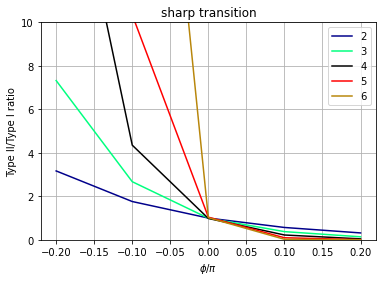
\includegraphics[width=1.0\textwidth]{ratioE12.png}
\caption[]{ 
 Plot of  ratios in  Table~\ref{tab:ratioE12},  $t = 10^{12}$.
 }
\vspace{1mm}, 
\label{ratioE12}
\end{figure*}

\begin{figure*}
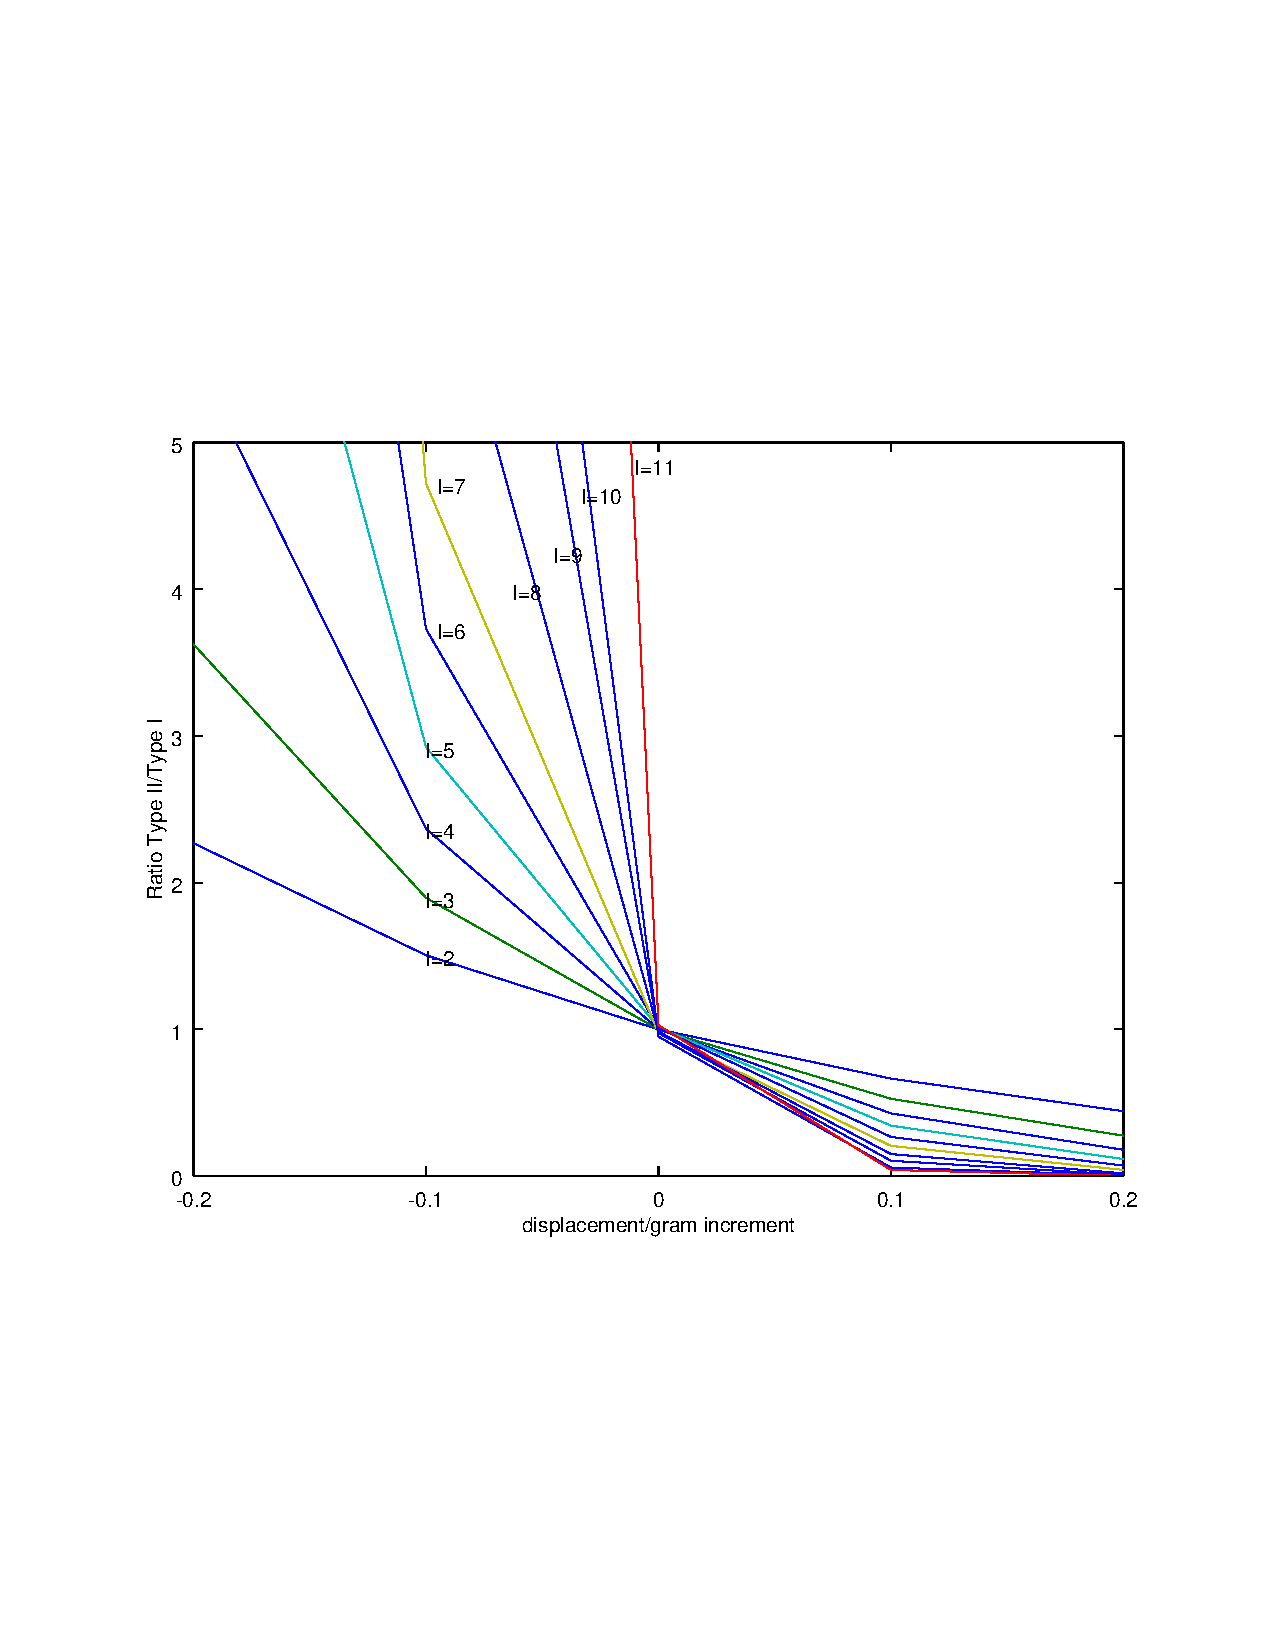
\includegraphics[width=1.0\textwidth]{typeIIratio.pdf}
\caption[]{ 
 Plot of  ratios in  Table~\ref{tab:ratioE28},  $t = 10^{28}$.
 }
\vspace{1mm}, 
\label{ratioE28}
\end{figure*}


\section{\label{conclusions}Conclusions}
Tables \ref{tab:ratioE12} and \ref{tab:ratioE28} show the sharp transition in the $Type~II/Type~I$ Gram block ratio.
Figures \ref{ratioE12} and \ref{ratioE28} show the sharp transition visually.
The ratio is greater than one and increases exponentially with the
Gram block length when $\phi$, the generalized Gram angle, is negative.
The ratio is lesser than one and decreases exponentially with the
Gram block length when $\phi$, the generalized Gram angle, is positive.
At the usual Gram points, the ratio is one, thus, there is a forward backward symmetry in the occurrence of Gram block patterns for the usual Gram points. The forward backward symmetry manifests itself in a more complex way~\cite{Shanker 2020}  for points away from the usual Gram points.

\begin{table}
\centering \(\begin{array}{cccccc}
\hline
Length~of  && Generalized &Gram&angle &\phi \\
Gram     &----&----&----&----&----\\
block  & -0.2\pi & -0.1\pi & 0.0\pi & 0.1\pi & 0.2\pi  \\
\hline
2 &3.167 &1.760 &1.000 &0.567 &0.316 \\
3 &7.323 &2.672 &0.993 &0.376 &0.138 \\
4 &20.958 &4.352 &0.982 &0.221 &0.043 \\
5 &170.829 &10.344 &1.041 &0.094 &0.008 \\
6 &1409.500 &35.516 &1.016 &0.023 &0.001 \\
\hline
\end{array}\)
\caption{Sharp transition in $Type~II/Type~I$ Gram block ratio.
The ratio is greater than one and increases exponentially with the
Gram block length when $\phi$, the generalized Gram angle, is negative.
The ratio is lesser than one and decreases exponentially with the
Gram block length when $\phi$, the generalized Gram angle, is positive.
The statistics are from $1$ million Gram intervals at $t=10^{12}$.}
\label{tab:ratioE12}
\end{table}

\begin{table}
\centering \(\begin{array}{cccccc}
\hline
Length~of  && Generalized &Gram&angle &\phi \\
Gram     &----&----&----&----&----\\
block  & -0.2\pi & -0.1\pi & 0.0\pi & 0.1\pi & 0.2\pi  \\
\hline
2 &2.269 &1.505 &0.999 &0.664 &0.441 \\
3 &3.625 &1.896 &0.999 &0.526 &0.275 \\
4 &5.589 &2.367 &1.001 &0.427 &0.178 \\
5 &8.850 &2.923 &1.012 &0.343 &0.115 \\
6 &14.373 &3.729 &1.009 &0.266 &0.071 \\
7 &23.962 &4.722 &0.975 &0.205 &0.041 \\
8 &51.791 &6.715 &0.984 &0.149 &0.018 \\
9 &116.632 &10.130 &0.975 &0.104 &0.009 \\
10 &361.615 &13.306 &0.949 &0.058 &0.005 \\
11 &1397.000 &34.533 &1.028 &0.041 &0.001 \\
\hline
\end{array}\)
\caption{Sharp transition in $Type~II/Type~I$ Gram block ratio.
The statistics are from $10$ million Gram intervals at $t=10^{28}$.}
\label{tab:ratioE28}
\end{table}


\section*{Acknowledgments and Funding Statement}

 The study was done as an independent researcher. There was no
external funding.

\section*{Ethical Compliance}

 No procedures were performed  involving human participants in the study.

\section*{Data Availability Statement}

The computer programs used during the current study are
available from the corresponding author on reasonable request.

\section*{Conflict of Interest declaration} 

The authors declare that they have no affiliations with or involvement in any organization 
or entity with any financial interest in the subject matter or materials discussed 
in this manuscript.


\bibliographystyle{amsplain}
\begin{thebibliography}{10}


\bibitem{Shanker 2018a} O. Shanker, 
``Good to Bad Gram Point Ratio For Riemann Zeta Function",
{\it Experimental Mathematics} {\bf 30}, 76-85,
\url{tinyurl.com/mwd5uwc5}(2021)

\bibitem{Shanker 2018b} O. Shanker, 
``Symmetry properties of distribution of Riemann Zeta Function values on critical axis''
 report,
\url{tinyurl.com/47wj57b3}, 
(2018). 

\bibitem{Odlyzko 1992}  A. Odlyzko,
``The $10^{20}$-th Zero of the Riemann Zeta
Function and 175 Million of its Neighbors", report,
\url{http://www.dtc.umn.edu/~odlyzko/unpublished/zeta.10to20.1992.pdf}, (1992)

\bibitem {Edwards(1974)} H. M. Edwards, ``Riemann's Zeta Function,''
Academic Press,  (1974)

\bibitem{osneural} O. Shanker, ``Neural Network prediction of Riemann zeta zeros''
{\it Advanced Modeling and Optimization}, {\bf 14}, 717-728, (2012), \url{tinyurl.com/4scve3nj}.


\bibitem{oscue} O. Shanker, 
``Random Matrix Theory explanation for Riemann Zeta Value Distribution Symmetry''
 report,
\url{https://tinyurl.com/ywhy4jsy}, 
(2022). 

\bibitem{os6} O. Shanker, 
``Generalised Zeta Functions and Self-Similarity of Zero Distributions",
{\it J.  Phys. A} {\bf39}(2006), 13983-13997

\bibitem{Shanker 2020} O. Shanker, 
``Universality of Riemann Zeta Function value distribution on critical axis''
 report,
\url{tinyurl.com/yvbd2je6}, 
(2020). 




\end{thebibliography} 

\end{document}
